\part{Rasterizer}


\section{Introduction}
Rasterization is an object order method. We have a list of objects in our scene and draw one after another. This is the opposite of an image order rendering technique, like raytracing, where each pixel is traversed. This is why raytracing can be slower than rasterization; -testing each pixel and, for each pixel, testing every object. This pipeline can require more computation than a rasterization pipeline, which is iterating over every object once and coloring the pixels the object occupies.

Raytracing can be accelerated by spatial sorting, like bounding volume hierarchies, but so can rasterization. Frustrum- and occlusion-culling are just two examples.

The most basic job of a rasterizer is to draw triangles using pixels on a raster display. A popular method is scaline rendering, because of cache locality and the way displays update their image a scaline at a time.

\begin{figure}[H]
  \centering
  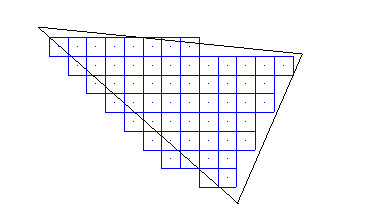
\includegraphics{Media/raster_scanline.png}
  \caption{Scanline rasterization of pixels}   
  \label{fig:Scanline rasterization of pixels}
\end{figure}